\documentclass[5p,times,procedia]{elsarticle}
\usepackage{float}
\usepackage{ecrc}
\volume{00}
\firstpage{1}
\journalname{Procedia CIRP}
\runauth{M.B. Jensen et al.}
\jid{procir}
\jnltitlelogo{Procedia CIRP}
\usepackage{amssymb}
\usepackage[figuresright]{rotating}
\usepackage[bookmarks=false]{hyperref}
\hypersetup{colorlinks, linkcolor=blue, citecolor=blue, urlcolor=blue}

\begin{document}
\begin{frontmatter}

\dochead{60th CIRP Conference on Manufacturing Systems (CIRP CMS 2027)}%

\title{From product requirements to running skills: AAS-driven planning and reconfiguration of IEC 61499 modules}

\author[a]{Martin B. Jensen\corref{cor1}}
\author[a]{Tristan Schwörer}
\author[a]{Casper Schou}

\address[a]{Aalborg University, Fibigerstræde 14, Aalborg 9220, Denmark}

\cortext[cor1]{* Corresponding author. {\it E-mail address:martinbj@mp.aau.dk}}

\begin{abstract}
Modular production systems must change their modules' behaviour as products change, yet a module's skills are fixed in its control program. This paper turns a product's requirement, stated in its Asset Administration Shell (AAS), into a new skill in a module's running IEC 61499 program. A product--process--resource model in the AAS lets products require capabilities with values and bounds and describes each module's skills down to its components' primitives, with capabilities derived from the skills and constrained by conditions, invariants and rates. A planner derives a composite skill from a requirement and the module's component capabilities, runs steps in parallel at rates it sets where a bound demands it, and checks the plan in time against the requirement. As composites are networks of primitive function block instances, a reconciler creates the new skill online, verifies it by reading the program back and records it. On a pharmaceutical filling module with Eclipse 4diac, a new skill is active within 0.7\,s while running skills continue and every drift between program and AAS is detected; against an independent process model, matching and planning are right in every case and the check finds 90\,\% of the flows that would spoil a product.
\end{abstract}

\begin{keyword}
Asset Administration Shell; IEC 61499; skill-based engineering; capability-based planning; reconfiguration; pharmaceutical manufacturing
\end{keyword}
\end{frontmatter}

\section{Introduction}
\label{sec:introduction}

Pharmaceutical production is moving from large batches on dedicated lines to small batches and personalised products. Frequent changeovers call for modular production systems, lines assembled from modules that are exchanged and reconfigured as the products change~\cite{schwoerer2025modular}. The Asset Administration Shell (AAS), the standardised digital twin of Industry~4.0, describes how a product and its requirements are modelled and what a module can do and how it is called. The description must also be reflected in the module's control program. IEC~61499~\cite{iec61499} makes this possible: a module's program is an event-driven network of function blocks, which management commands create, connect and parameterise in the running device without stopping the parts that do not change~\cite{rooker2007zero}. In aseptic filling, for example, a vial is filled with the needle at a fixed depth, whereas a prefilled syringe is filled from the bottom of its barrel, the needle rising with the liquid while the pump doses. Needle and pump stay the same; the new behaviour joins them in one skill, their speeds matched to the syringe. How a product's AAS can drive such a change of a module's program has not been investigated.

Skill-based engineering separates what a resource can do, its capability, from how it is done, its skill~\cite{koecher2023reference}, and the AAS describes both, for instance in the Capability Description~\cite{idta02020}. Most work composes skills from above and takes each skill as given: a workflow engine invokes the devices' skills~\cite{lindorfer2019user}, planners sequence the skills that resources already have~\cite{nabizada2026capability,koecher2024smt}, behaviour trees call the modules' skills through their AASs~\cite{jensen2026service,schwoerer2026fond}, and generated orchestrators call the skills of stations~\cite{dorofeev2021orchestrator}. The skill they call is a black box in the device's code, and a new behaviour inside it needs the vendor's engineering project, an IDE and a redeployment. In this paper a module's skills are networks of hardware-near primitives~\cite{schou2018skill}, such as moving the needle, dosing and weighing, in standard IEC~61499 on the device itself, so that a new skill can be planned from a product's requirement and created in the running program.

The contributions are:
\begin{itemize}
\item[(C1)] a product--process--resource model in the AAS that joins a product's required capabilities, a module's composite skills and its components' primitives through capabilities derived from the skills and constrained in a form a planner can use;
\item[(C2)] a planner that derives a composite skill from a requirement the module does not offer, including steps that must run in parallel at matched rates, and checks it in time before deployment;
\item[(C3)] the deployment of the new skill: a module architecture in which composites are networks of function block instances, and a reconciler that creates them online, verifies them by reading the program back and records them in the AAS.
\end{itemize}
They are evaluated with Eclipse 4diac on a pharmaceutical filling module.

\section{Related work}
\label{sec:related}

Four lines of work meet here (Table~\ref{tab:related}). \emph{Composing skills on controllers.} Dorofeev et al. generate a composite skill as IEC~61499 code from a given orchestration sequence~\cite{dorofeev2021orchestrator}; this cut the engineering effort in 4diac by a factor of 2.7 to 5.5, but yields a basic function block whose state machine grows to $2^n$ states for $n$ parallel skills, and keeping the skill descriptions in the AAS is their future work. Terzimehić et al. compute the services' deployment with SMT from a recipe, the plant topology and component models, and generate an IEC~61499 application~\cite{terzimehic2021service}. Lindorfer and Froschauer validate BPMN skill sequences against a rule set before an external workflow engine runs them~\cite{lindorfer2019user}. In all three, a composition is made at engineering time and never read back from the running program.

\emph{The AAS as a source for control.} The AAS describes offered capabilities with their constraints and skills with their endpoints, and a product's features are matched against them~\cite{blumhofer2025enhancing}; how a skill is composed stays inside the machine. Albus et al. derive a bill of process from a product's CAD model, match it against the resources' capabilities and let agents orchestrate the resources' skills~\cite{albus2025automated}, noting that new processes otherwise need manual integration into the control system. Both select and call existing behaviour. \emph{Changing IEC~61499 programs online.} Reconfiguration services keep an application running while a part changes~\cite{rooker2007zero}. Huang et al. turn a Module Type Package file, compared with what runs, into management commands within 96\,ms~\cite{huang2026plug}; the orchestration is still redrawn by hand, and the result is not checked against the file afterwards.

\emph{Planning from capabilities.} PDDL is generated from capability models in the AAS~\cite{nabizada2026capability}, and policies planned from distributed AAS descriptions run as behaviour trees~\cite{schwoerer2026fond}. Köcher et al. plan processes from a capability ontology with SMT, allowing parallel capabilities within one step but no durations or continuous change~\cite{koecher2024smt}. These sequence or assign skills that exist; none turns a plan into a new skill of the resource, or plans what must happen at the same time. \emph{Gap.} No approach takes a product's requirement in the AAS to a new skill that is planned from the module's capabilities, checked in time, created in the running IEC~61499 program and verified by reading it back.

\begin{table}[t]
\centering
\caption{The closest works. AAS: the AAS describes the new behaviour; Plan: it is planned from a requirement; 61499: it runs in the controller's IEC~61499 program; Online: it is changed online; Check: it is checked before deployment; Read: the running program is compared with its description. \checkmark~yes, (\checkmark)~in part, --~no.}
\label{tab:related}
\footnotesize
\setlength{\tabcolsep}{2.2pt}
\begin{tabular}{@{}llcccccc@{}}
\hline
Work & New behaviour from & AAS & Plan & 61499 & Online & Check & Read \\
\hline
\cite{dorofeev2021orchestrator} & a given sequence & -- & -- & \checkmark & -- & -- & -- \\
\cite{terzimehic2021service} & recipe, SMT & -- & (\checkmark) & \checkmark & -- & (\checkmark) & -- \\
\cite{lindorfer2019user} & BPMN by the user & -- & -- & -- & -- & \checkmark & -- \\
\cite{huang2026plug} & MTP file & -- & -- & \checkmark & \checkmark & -- & (\checkmark) \\
\cite{blumhofer2025enhancing} & product features & \checkmark & -- & -- & -- & (\checkmark) & -- \\
\cite{albus2025automated} & CAD model & -- & (\checkmark) & -- & -- & (\checkmark) & -- \\
\cite{koecher2024smt} & capability ontology & -- & \checkmark & -- & -- & (\checkmark) & -- \\
Ours & product's requirement & \checkmark & \checkmark & \checkmark & \checkmark & \checkmark & \checkmark \\
\hline
\end{tabular}
\end{table}

\section{Method}
\label{sec:method}

\subsection{Overview}
\label{sec:overview}

A product's requirement passes through three steps (Fig.~\ref{fig:concept}). The product's AAS states the capabilities its processes require; matching compares them with the capabilities the modules offer and answers offered, not offered, or offered after a reconfiguration. Where nothing fits, the planner derives a new composite skill from the module's capabilities and describes it in the module's AAS, which is the desired state of the module's program; the reconciler then makes the running program equal to it, online where the change allows. The AAS is the source because every module comes with it and every client reads it~\cite{jensen2026service}, whereas code generators start from engineering models~\cite{dorofeev2021orchestrator,terzimehic2021service} that an integrator seldom has. Behaviour has three levels, as device primitives, skills and tasks do in~\cite{schou2018skill}: components offer primitive skills, a module composes them, and the line, outside this paper, orchestrates the modules.

\begin{figure*}[t]
\centering
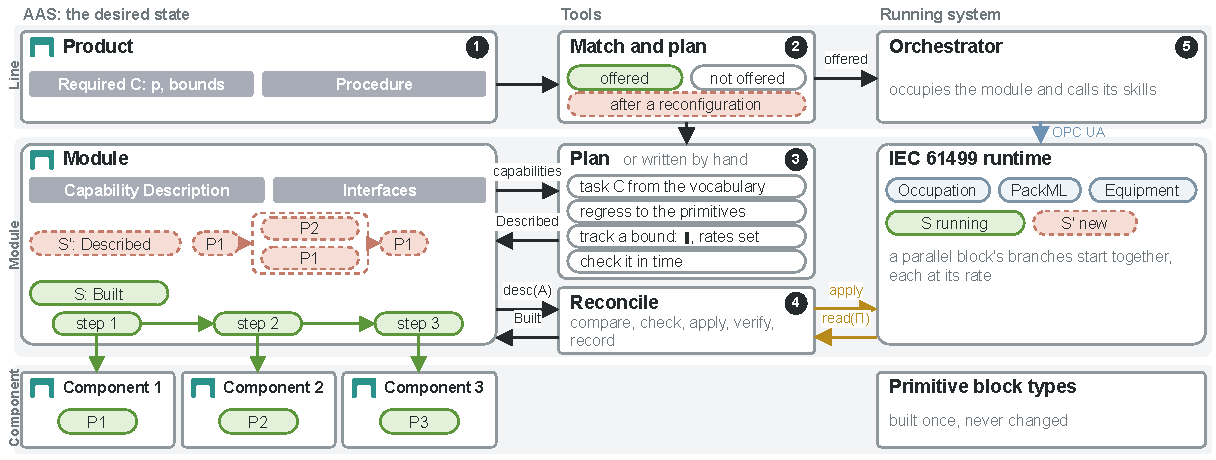
\includegraphics[width=\textwidth]{figures/pipeline-planning.pdf}
\caption{From a product's requirement to a running skill, on three levels. (1)~A product requires a capability C with parameters p and bounds, and (2)~matching answers offered, not offered, or offered after a reconfiguration, and plans what nothing offers. (3)~The planner derives a skill S$'$ from the module's capabilities and the vocabulary, with a parallel block where a bound requires it, checks it in time and describes it. (4)~The reconciler applies it online, reads the program back and records it as Built. (5)~The orchestrator calls the skills over OPC~UA. Gold: change over the management protocol; blue: operation; green: a step runs a primitive.}
\label{fig:concept}
\end{figure*}

\subsection{The product--process--resource model in the AAS}
\label{sec:model}

\emph{Skills.} Primitives are described in their component's AAS and composites in the module's, in a Skills submodel. A skill's commands are Operations whose inputs are its parameters, with unit, limits, default and meaning, and whose outputs are its results; each refers to the action of the Asset Interfaces Description that calls it. A composite's Start command holds its flow: steps that refer to the components' primitives, with bindings of constants and parameters, parallel blocks and decisions, block-structured so that every flow maps to blocks (Section~\ref{sec:deploy}).

\emph{Capabilities.} The module's Capability Description~\cite{idta02020} holds one capability set per component, each capability realized by a primitive and constrained by basic constraints: preconditions, postconditions and invariants, whose operands may be linear formulas of the capability's properties. A property may be the rate of another. Dosing thus has a precondition that the needle is at the fill position or deeper, a postcondition that the container's content grows by the dosed volume at the pump's flow rate, and invariants that keep the needle below the container's rim and define how deep the needle is in the liquid,
\begin{equation}
d = y - (z_n - h_b) + V/A,
\label{eq:depth}
\end{equation}
where $y$ is the needle's position down its axis and $z_n$ that of the nest, the module's facts, $h_b$ the height of the container's inner bottom above the nest and $A$ its inner cross-section, the product's facts, and $V$ the volume in it. Positioning moves the needle to a given position at the axis's speed and keeps it above the container's inner bottom. The offered capabilities are derived from the skills. Each primitive's type realizes a capability of its component and contributes one to the composites that run it: Dispense realizes dosing, an auxiliary capability, and contributes filling, a process capability. A composite offers the process capabilities its steps contribute, specified by the properties its parameters mean, with ranges found by running it through the module's states, so that two doses of 0.5--10\,mL offer 1--20\,mL.

\emph{Meanings.} Every capability and property carries its meaning as a supplemental semantic identifier from a shared vocabulary. It separates process capabilities, which a product can require, from auxiliary ones, which serve other skills, places them below the classes of DIN~8580 and VDI~2860 where these fit, states which property is the rate of which, and defines narrower capabilities by constraints: bottom-up filling is a filling that keeps the needle within bounds of the liquid's surface.

\emph{Products and processes.} A product's process step requires a capability with values (a fill volume), bounds (how far the needle may be from the surface) and the product's facts (the container's geometry). Matching compares the meaning of the required capability with the offered ones and each required value with the offered range in the same unit; a capability with constraints is then checked against the requirement (Section~\ref{sec:plan}). It answers offered, not offered, or offered after a reconfiguration, by a skill that is \emph{Described} but not yet \emph{Built}, and the process AAS binds the step to the module and the skill. Albus et al. match a product's requirements against capabilities to assign existing skills~\cite{albus2025automated}; here a requirement nothing meets leads to a new skill.

\subsection{Planning a composite skill from a requirement}
\label{sec:plan}

\emph{The request.} In the process planner, one command goes through a product's steps. A step whose requirement a skill matches is bound to it; a skill whose capability states constraints is first checked against the requirement; otherwise a skill is planned on a module that the matching names as able to carry the capability out, or that offers a capability the required one narrows. No module type is needed: what a module can do is what its capabilities say.

\emph{The planner.} The planning domain is read from the module's Capability Description, an action per component capability, and the task from the vocabulary's class with the requirement's values. The planner combines hierarchical task networks with goal regression~\cite{nau2021gtpyhop}. The task's goals are its postcondition, what the results asked for need, such as a weight once the container is weighed, and the module's rest state. A goal, such as the content reaching 1\,mL, is reached by the compositions the module states, if any, else by an action whose postcondition achieves it, after its own preconditions, which become goals in turn; a volume above one dose is split into equal doses. Every action must keep its own invariants and the requirement's at its start and its end. Between two events, a step starting or ending, every state $s$ changes at a constant rate $\dot{s}$, so a quantity linear in the states, $g = c^\top s + c_0$, changes linearly,
\begin{equation}
g(t) = g(t_k) + (t - t_k)\, c^\top \dot{s}, \quad t_k \le t \le t_{k+1},
\label{eq:linear}
\end{equation}
and a bound on $g$ that holds at $t_k$ and $t_{k+1}$ holds in between. An action that breaks a bound is not applied, and the planner backtracks to its next method.

\emph{Steps at the same time.} Where an action that changes a state at a rate would break a bound on a quantity that a formula defines, a second method pairs it with an action that moves another state of that formula. It sets the rate that can be set so that the quantity stays constant, $c^\top \dot{s} = 0$ in Eq.~(\ref{eq:linear}), and first brings the other state to the middle of the range that every bound leaves at the start and the end (Fig.~\ref{fig:plan}). For the depth $d$ of Eq.~(\ref{eq:depth}), the pump changes $V$ at its flow rate $r$ and the axis moves the needle up at its speed $v$, so $d$ stays constant when $r/A - v = 0$: as the axis's speed is fixed, the pump is set to $r = Av$, 0.396\,mL/s for the syringe's 31.7\,mm$^2$ at 12.5\,mm/s. For 1\,mL, the needle starts 1.5\,mm above the barrel's bottom and rises 31.6\,mm in 2.53\,s. The pair becomes a parallel block when the plan is lifted to a partial order, in which steps on different components with no state between them run in parallel too. Köcher et al. allow parallel capabilities within one step and leave durations to future work~\cite{koecher2024smt}; PDDL generated from planning submodels~\cite{nabizada2026capability} adds planning-specific elements to the AAS, whereas here the standard constraints suffice.

\emph{The check.} Every flow, planned or handcrafted in a skill editor, is checked before it is described. It is run through the module's capabilities from the product's state, event by event where its steps' durations are known, which is exact for linear constraints without time steps, and a condition that fails is reported with its step and a step that would make it hold. Where Lindorfer and Froschauer check rules written by an expert~\cite{lindorfer2019user}, the rules here are the capabilities' constraints already in the AAS. Only a skill that keeps the requirement is described and offered after a reconfiguration.

\begin{figure}[t]
\centering
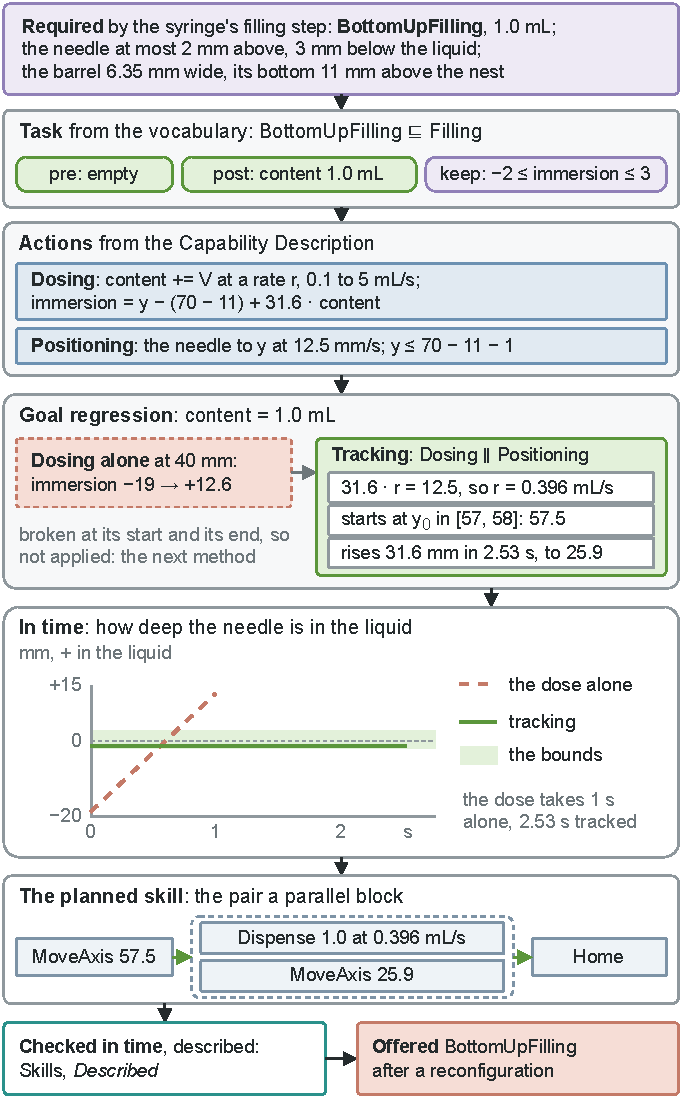
\includegraphics[width=\columnwidth]{figures/planned-bottom-up.pdf}
\caption{Bottom-up filling planned for a syringe from the filling module's capabilities: the requirement and the task from the vocabulary; the actions, with their rates and the formula for the needle's depth in the liquid; dosing alone refused, as it breaks the bound; the tracking that sets the flow rate and the needle's start; the depth over time; and the planned skill with its parallel block.}
\label{fig:plan}
\end{figure}

\subsection{Deploying the skill on the module}
\label{sec:deploy}

The program follows fixed rules that make a composite skill data rather than code. A shell, the same in every module and never changed online, holds an occupation that lets one client at a time command the module, a PackML state machine and one block per equipment item that owns its IO. A primitive skill is a block type built into the runtime once; every skill has the same small state machine and the same OPC~UA methods (Start, Stop, Abort, Reset), its parameters being the arguments of Start, range-checked before anything moves. A composite has no type of its own: it is a subapplication of instances, a block for its state machine and methods, a latch per parameter and an instance of a primitive per step, named like the step and holding its constants. Steps are chained by their success events, and a parallel block adds a join. The rules derive all wiring from the flow, so that a skill, a step and a parameter in the AAS are, by name, a subapplication, an instance and a latch in the program. Instances are used because every IEC~61499 runtime creates them online through management commands~\cite{iec61499}, while a new type needs a build, and because a generated type grows to $2^n$ states for $n$ parallel branches~\cite{dorofeev2021orchestrator} where a join grows linearly. Blocks reach the equipment over the runtime's local publish/subscribe channels, so a new composite needs one connection to what runs: zero downtime holds by construction.

A change falls into one of three classes. A \emph{parameter} change is written online while the module is neither executing nor occupied; a \emph{flow} change that adds a composite is made online in any state, while reordering or removing one needs a restart; a \emph{structural} change, a new primitive or IO, needs a build.

Let $\Pi$ be the running program and $A$ the module's AAS. The reconciler reads $\Pi$ back over the management protocol, which reports every instance, connection, type hash and value, and parses it by the rules into skills, steps, constants and types, $\mathit{read}(\Pi)$; the AAS gives the same structure, $\mathit{desc}(A)$. The module is verified when
\begin{equation}
\mathit{read}(\Pi) = \mathit{desc}(A).
\label{eq:verify}
\end{equation}
Otherwise the differences are sorted into the three classes. The reconciler checks that the steps name primitives the module has and that the values lie within their limits, applies what the class allows online by management commands, and refuses the rest as needing a restart or a build. It then reads the program back to evaluate Eq.~(\ref{eq:verify}) again, adds the change to the boot file, and marks the skill Built in the AAS. Huang et al. compare the runtime with the file before sending commands~\cite{huang2026plug}; reading back afterwards also reveals a command that was lost or refused. As the commands that create a composite come from the generator's own function, a program changed online equals one generated with the skill.

\section{Evaluation}
\label{sec:evaluation}

The filling module has a needle on a linear axis, a pump and a scale. Its program was generated by the rules and runs on Eclipse 4diac FORTE 3.3.0 on a PC with simulated IO. One patch lets the runtime's management answers be read in parts, so that programs of more than about 600 connections can be read back, and the event lists were raised to 1,024. Medians are given with 95\,\% intervals.

\emph{Deployment (C3).} New composites of 1 to 32 steps were added to programs of 1 to 20 composites, and values were changed, 30 runs per cell in random order, 1,260 runs in all, against redeployment by a new boot file and a restart. Every run passed every check, among them a comparison with the program the generator makes from the AAS. A composite of 32 steps in a program of 20 is active in 0.396\,s [0.387, 0.414], and the slowest of 780 additions took 0.664\,s (Fig.~\ref{fig:activation}); the time grows by 0.14\,ms per command and 0.21\,ms per connection read back. The commands were those of the generator's boot files in all 1,020 online runs, 73 for one step to 716 for 32. A skill running meanwhile took $-0.02$\,\% [$-0.08$, 0.04] longer. A restart leaves the module unavailable for 3.3\,s, 2.6\,s of it homing the axis; a new composite added online, not at all. A value changed between orders takes 0.03 to 0.24\,s online; changed during an order, the module must stop and reset first, and online is only 1.3 to 1.4 times faster than a restart. For consistency, nine kinds of drift were made in the program (a value written, a connection deleted, a stray instance, a reconfiguration cut after any of its commands, a type version) and in the AAS (a value, a step added, a flow reordered, a skill removed), 1,258 runs in all (Table~\ref{tab:results}). The reconciler detected and located every drift without a false alarm, removed those of an online class and refused the others; a cut reconfiguration was completed after any of its 135 commands. Comparing the AAS with the deployed boot file instead, as a deployment that does not read back would, found none of the 937 drifts made in the program.

\begin{figure}[t]
\centering
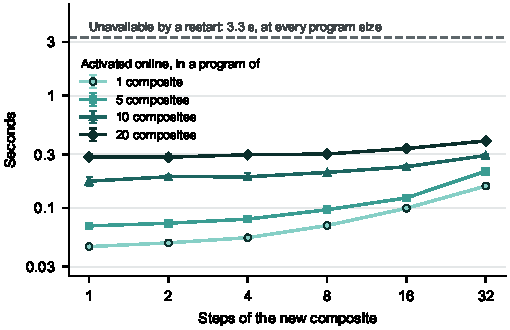
\includegraphics[width=\columnwidth]{figures/activation.pdf}
\caption{Deployment: the time from the AAS to the verified program for a new composite, against its number of steps, for programs of 1 to 20 composites (medians of 30 runs; the intervals lie within the markers). The module keeps running; a restart leaves it unavailable for 3.3\,s.}
\label{fig:activation}
\end{figure}

\emph{Model, check and planning (C1, C2).} The truth came from a process model of the station that uses none of the AAS's constraints: the needle's depth, the liquid in the container, spills and the weight, run in 10\,ms steps. All 245 single mutants of three skills (a step deleted, swapped, duplicated or inserted, a value changed or beyond its limit, two steps made parallel) were checked; 136 spoil the product. The check rejected 123 of them (recall 90\,\%) at a precision of 88\,\%, against 75\,\% recall for hand-written sequence rules and 2\,\% for the structural check an IDE makes. It misses a tare inserted after filling has begun, for which no condition exists, and refuses some flows the physics allows, such as weighing with the needle at home where out of the container suffices. For 26 products (vials and a syringe, 0.25 to 25\,mL, with or without their weight) on four module variants, the answer offered, offered after a reconfiguration or not offered equalled the process model's in all 104 cases, and nothing was offered that the module cannot do; all 23 planned skills made the product right the first time. For a syringe filled from the bottom with the needle at most 2\,mm above and 3\,mm below the liquid, 15 of 24 cases were planned, all with the needle rising alongside the dose, and all were right in the process model; the other 9 are those the module cannot do. Planning took 2.4\,ms (median) for the vials and 39\,ms for the syringe, where dosing alone is tried first, and checking a flow 1.8\,ms. A person's inputs for a change, by hand in 4diac, in the skill editor and with the planner, are in Table~\ref{tab:results}: the planner needs 6 inputs for a skill that takes 71 in 4diac, and deploying takes one online command instead of a restart.

\begin{table}[t]
\centering
\caption{Results on the filling module.}
\label{tab:results}
\footnotesize
\setlength{\tabcolsep}{3pt}
\begin{tabular}{@{}lll@{}}
\hline
Question & Measure & Result \\
\hline
Drift (1,258 runs) & detected and located & 1,157 of 1,157 \\
 & false alarms, clean runs & 0 of 101 \\
 & removed online, refused & 572, 577 \\
 & by the boot file instead & 220 of 1,157 \\
Check (245 mutants) & recall, precision & 90\,\%, 88\,\% \\
 & recall: rules, structure & 75\,\%, 2\,\% \\
Matching (104 cases) & equal to the process model & 104 of 104 \\
 & planned skills right & 23 of 23 \\
Bottom-up (24 cases) & planned, right & 15, 15 \\
Inputs: 4diac, & a value & 3, 4, -- \\
\quad editor, planner & a second dose & 55, 14, -- \\
 & bottom-up filling & 60, 25, -- \\
 & a 15\,mL product & 71, 14, 6 \\
\hline
\end{tabular}
\end{table}

\section{Discussion}
\label{sec:discussion}

What makes the AAS necessary here is the planner. A skill editor that writes a composite from a drawn flow comes close to generating an orchestrator from a given sequence~\cite{dorofeev2021orchestrator}; deriving the flow from a product's requirement needs what the AAS adds: the requirement with its values and bounds, the components' capabilities with their conditions and rates, and a vocabulary that says which capability narrows which. The effort points the same way. Dorofeev et al. report 2.7 to 5.5 times less effort than writing the code in 4diac~\cite{dorofeev2021orchestrator}; here a new skill takes 2.4 to 5 times fewer inputs in the skill editor than in 4diac, and 12 times fewer with the planner where it applies, though the two studies count different things.

Nothing in the planner, the check or the reconciler is about filling: the needle, the liquid and the container are data in the vocabulary and in the module's and product's AASs. The pairing of rates applies wherever one rate must follow another, such as a bead of adhesive laid along a path or a part taken from a moving conveyor, but it was evaluated on filling only.

The process model was written apart from the AAS's constraints, though by the same authors. For the syringe, the 2\,mm bound is the same number in the requirement and in the model's foam rule, so agreement there shows that planning and checking keep a stated bound over time, not that the bound is right; the 3\,mm bound is kept by the planner alone. The check's misses and excess point to the module's model rather than to the method: a condition on taring could catch the 13 misses, and a condition for weighing relative to the rim could remove 14 of the 17 refusals. Online is not always faster: a value changed during an order needs the module stopped and reset, and reordering or removing a composite needs a restart, as it deletes instances a running skill may hold.

\section{Conclusion}
\label{sec:conclusion}

A product's requirement in its AAS was taken to a new skill running in a module's IEC~61499 program, through a product--process--resource model in the AAS, a planner that derives composite skills from the module's capabilities, and a reconciler that deploys and verifies them online. A new skill was active within 0.7\,s while the module kept running, every drift between program and AAS was found, and matching and planning were right in every case against a process model that knows none of the AAS's constraints, while the check found 90\,\% of the flows that would spoil a product; the planner placed steps side by side at rates it set where a bound required it. The evaluation ran on a PC with simulated IO and one module type; a planned skill holds the values of the requirement it was planned for, and one quantity is tracked at a time. Next, the line's agents will request such plans themselves.

\bibliographystyle{elsarticle-num}
\bibliography{references}

\end{document}
